\section{Results}
\label{sec:results}

The limits shown in this section are obtained with the Higgs Combination tool, with the Asymptotic method. 
It has been noticed in the analysis that the central expected values can change by up to $15\%$ when running the full CLs method. 
The full CLs method, however, takes considerably longer to run, therefore, the full CLs limits did not get ready for the freezing deadline. 

Figure~\ref{fig:result_radion} shows the results on spin-0 resonances.
%Figure~\ref{fig:result_graviton} shows the results on spin-2 resonances.  
Figures~\ref{fig:nonres} (in fb) and \ref{fig:nonres_norm} (normalized to SM cross section) show the
SM-like non-resonant limit and its breakdown in the different analysis
categories: LM (Low Mass), HM (High Mass), MPC (Medium Purity
Category), and HPC (High Purity Category).

\begin{figure*}[h]
  \centering
  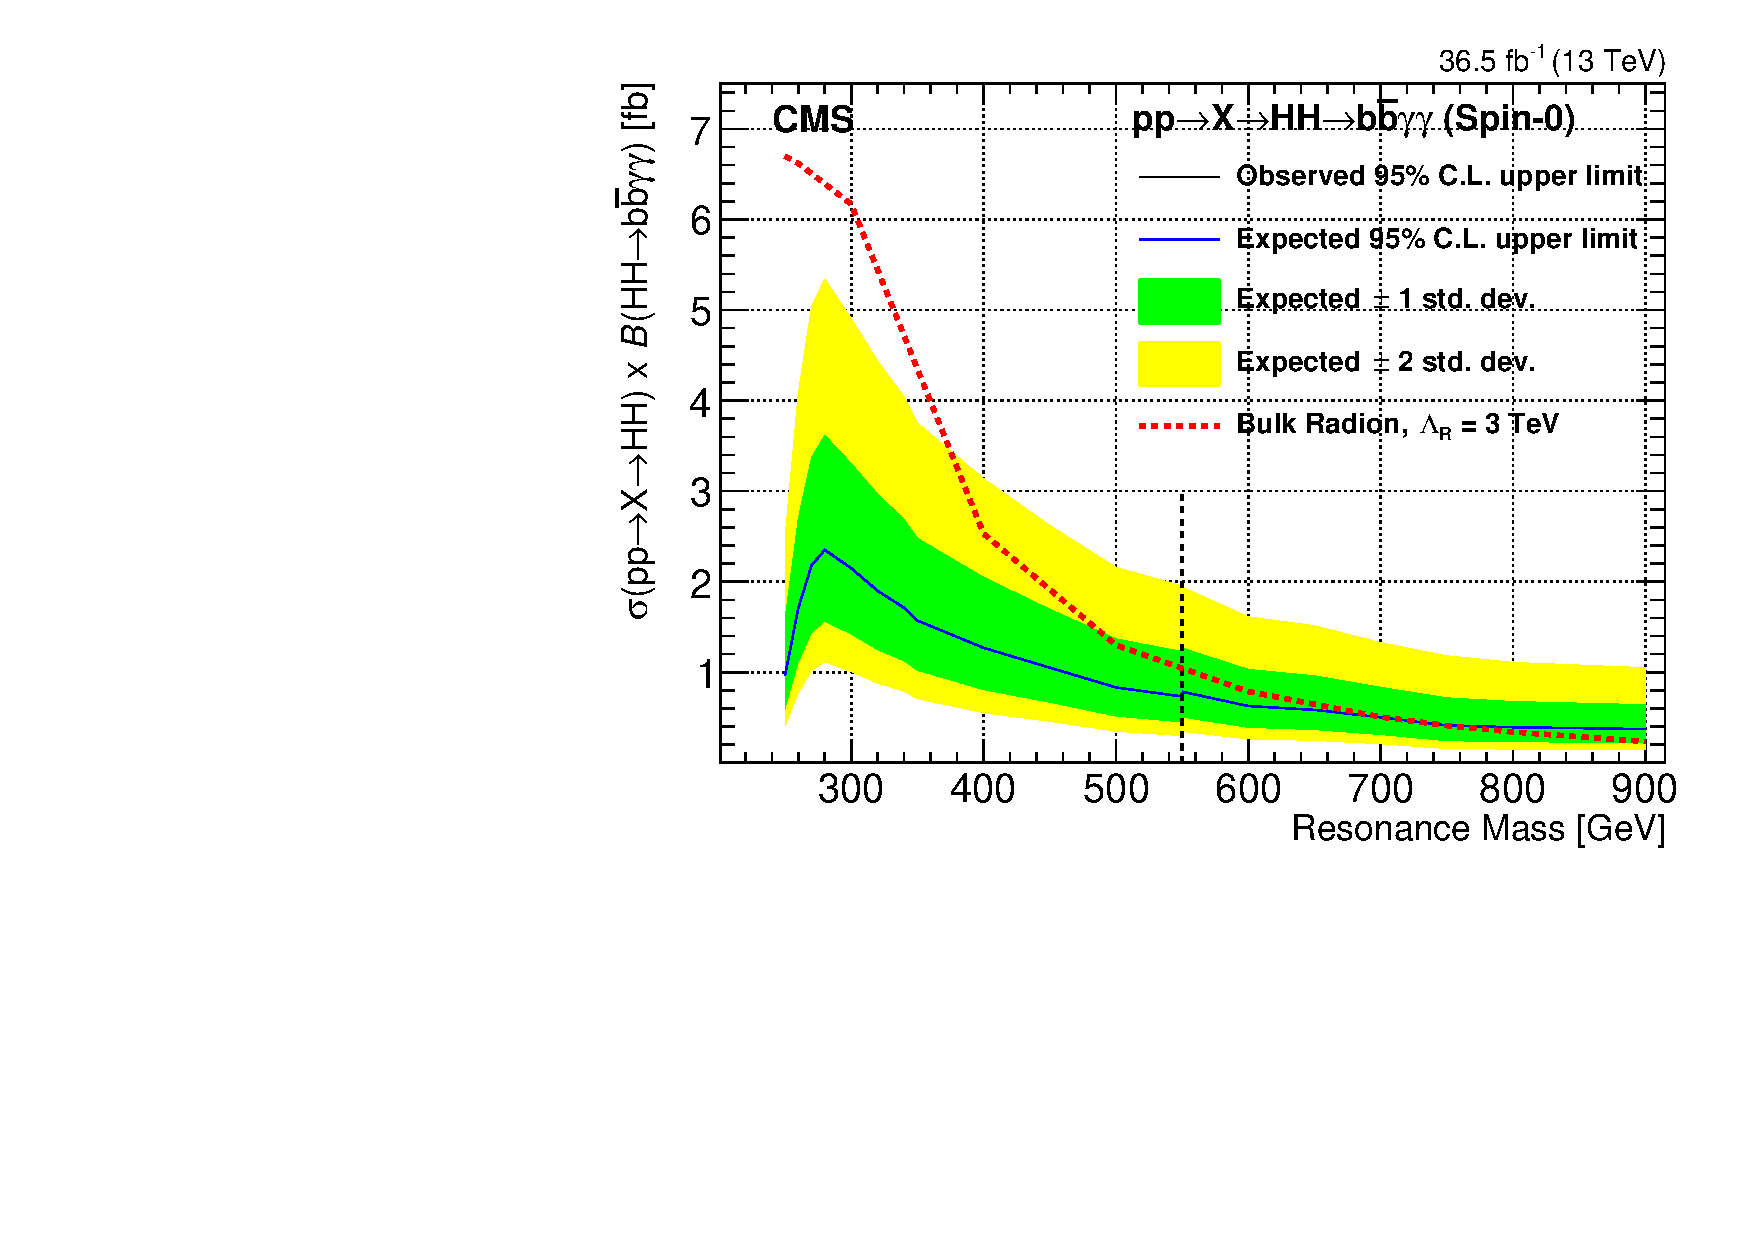
\includegraphics[width=0.7\textwidth]{figures/sec-results/LimsRadionLMHM.pdf}\hfil
  \caption{Limits on spin-0 resonances.}
  \label{fig:result_radion}
\end{figure*}

\begin{figure*}[h]
  \centering
  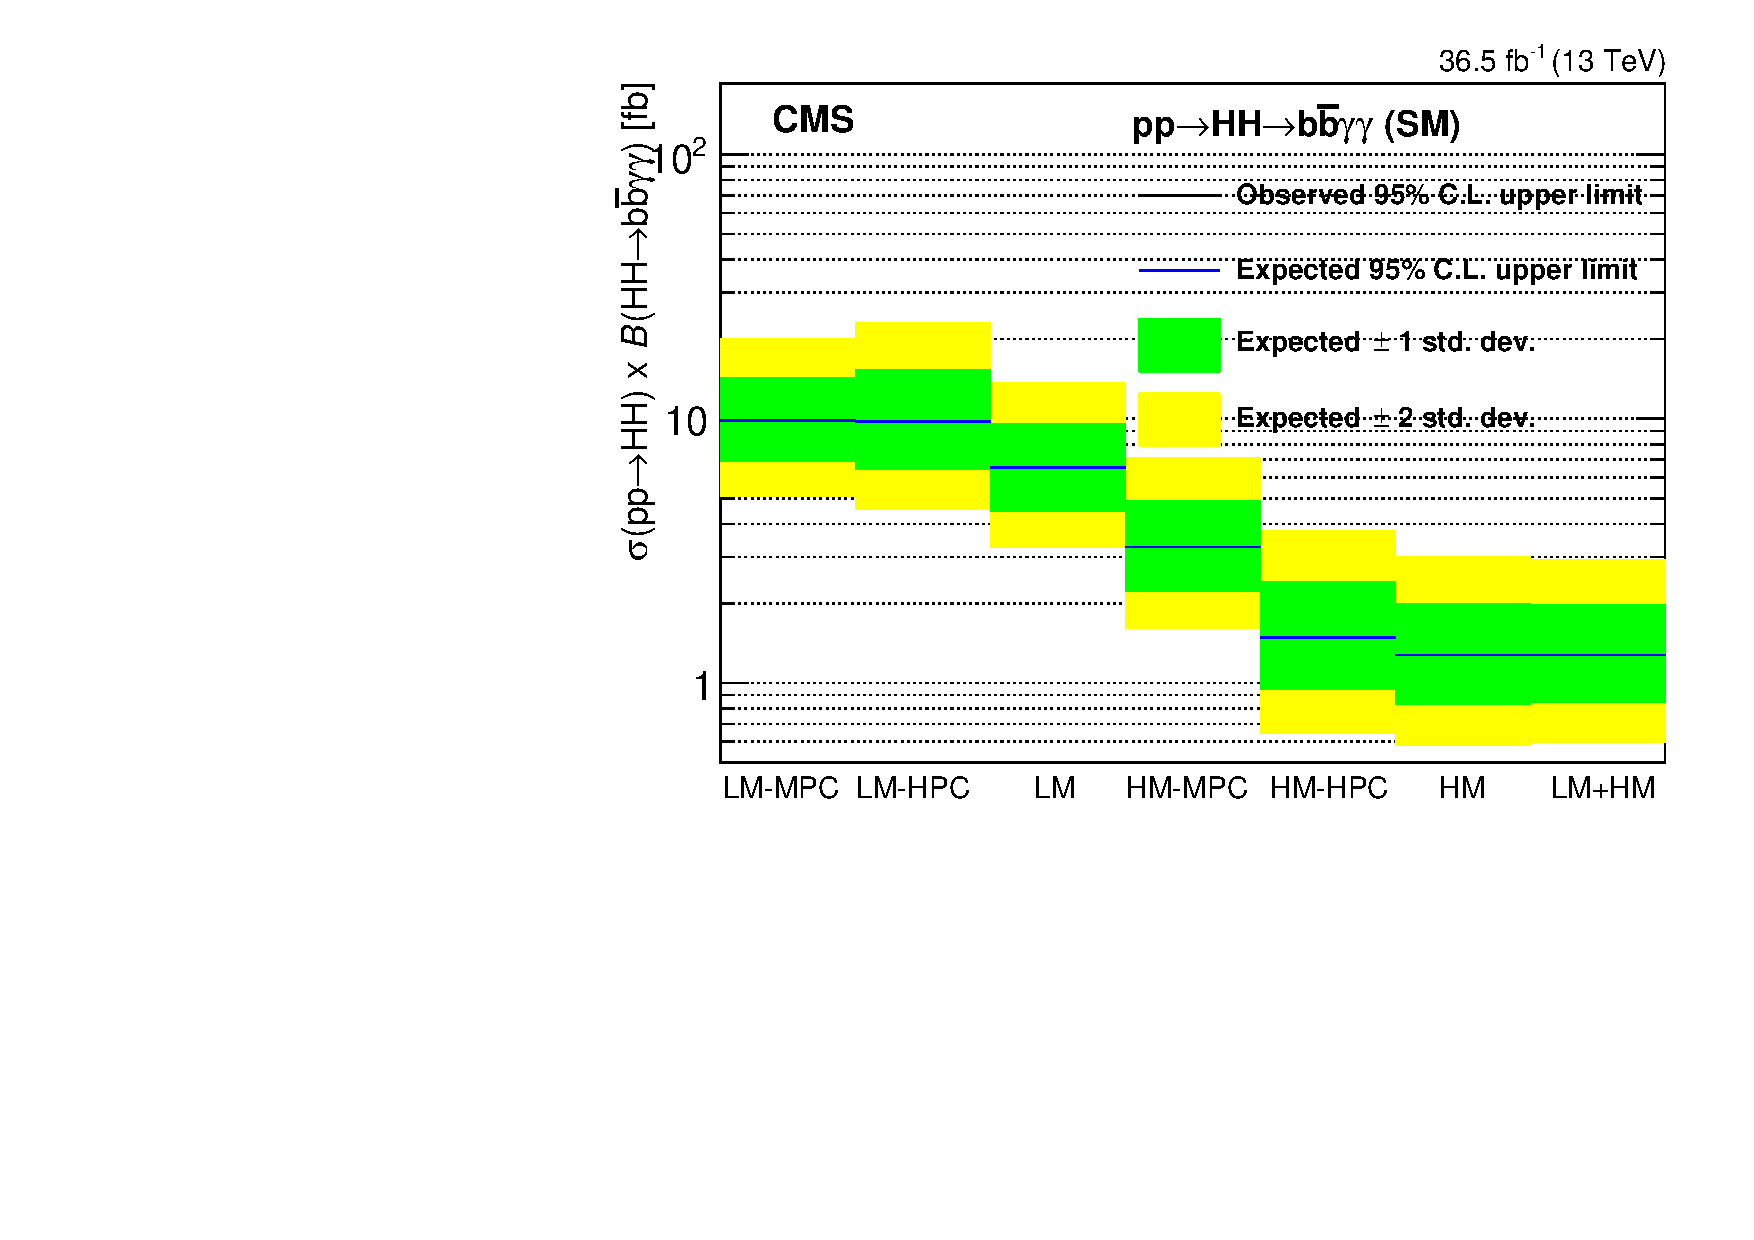
\includegraphics[width=0.7\textwidth]{figures/sec-results/NonResSMCats.pdf}\hfil
  \caption{SM-like non-resonant limits.}
  \label{fig:nonres}
\end{figure*}

\begin{figure*}[h]
  \centering
  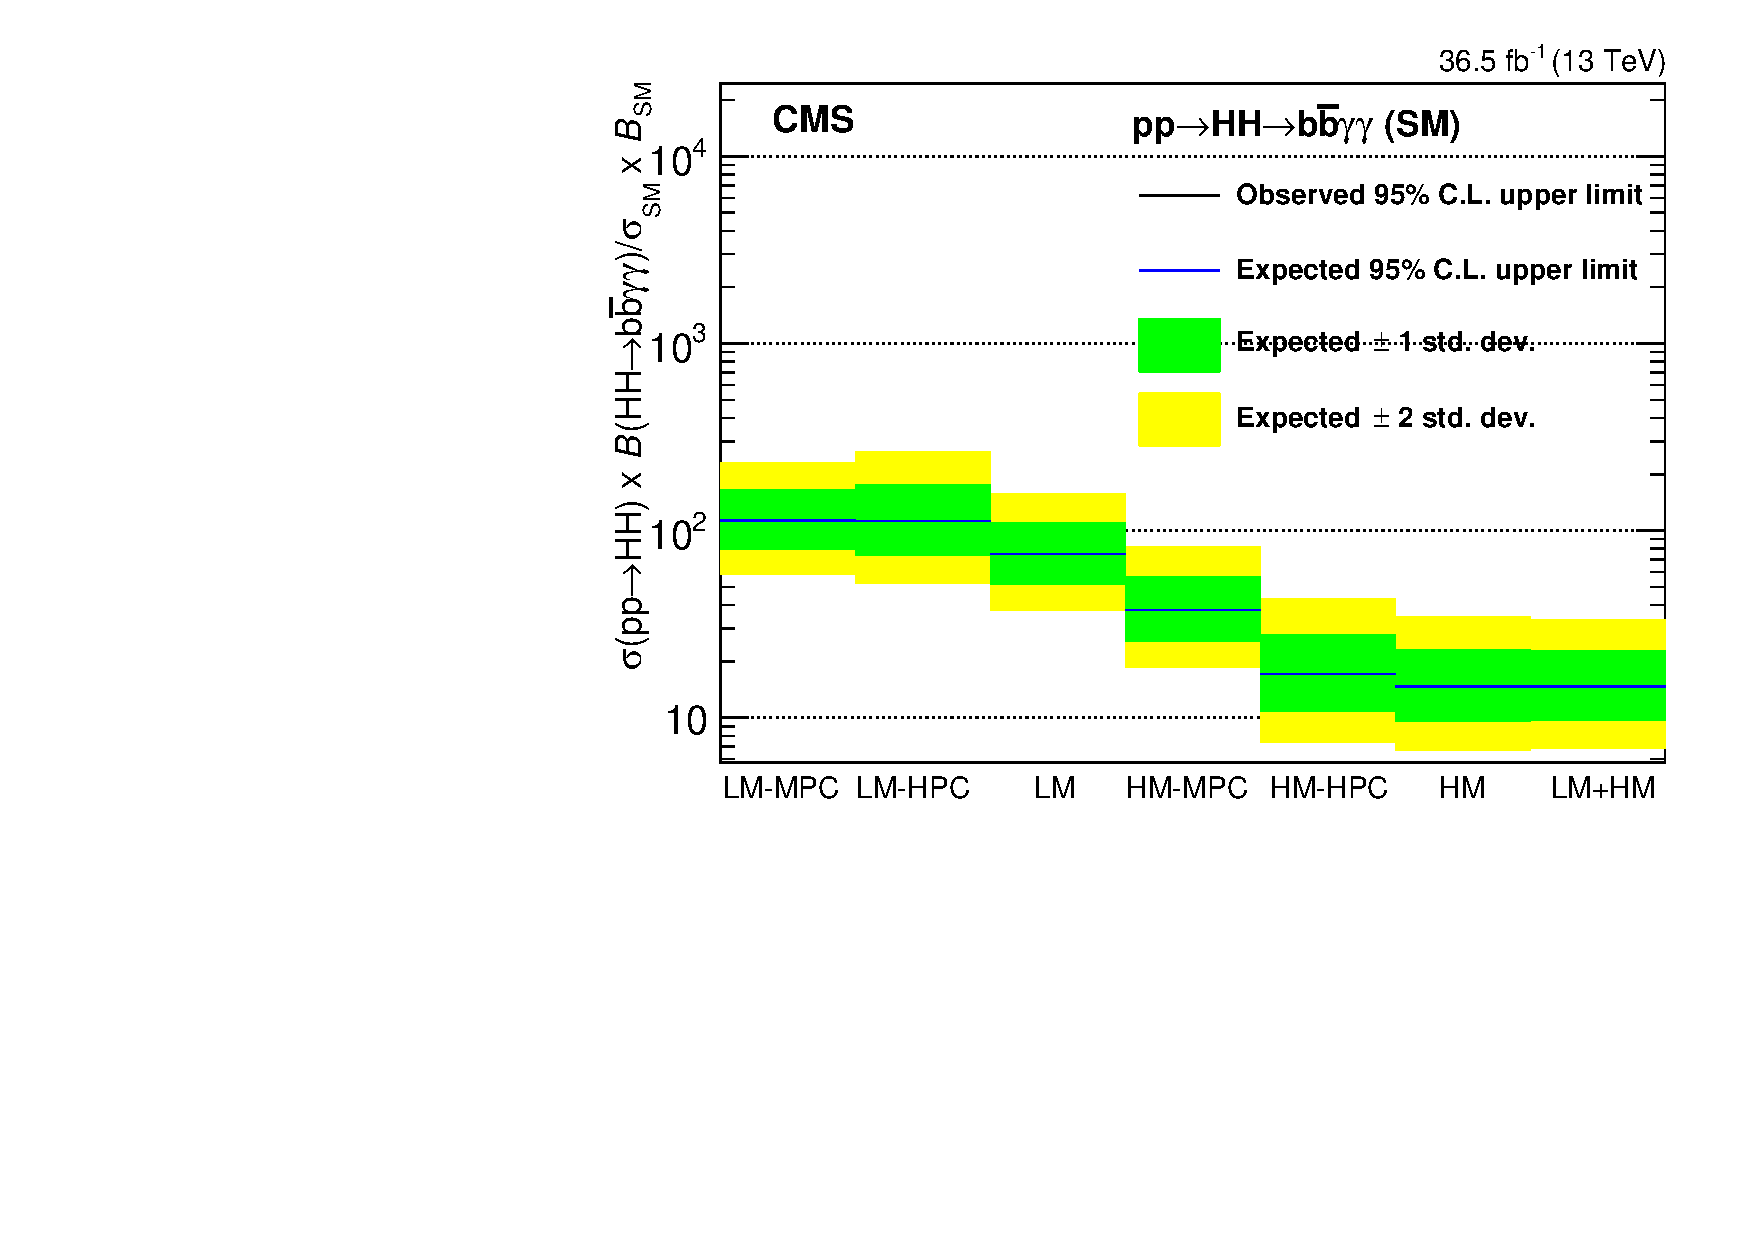
\includegraphics[width=0.7\textwidth]{figures/sec-results/NonResSMCats_SM.pdf}\hfil
  \caption{SM-like non-resonant limits normalized to SM cross section.}
  \label{fig:nonres_norm}
\end{figure*}
